% =============================================================================
% File        : presentation.tex
% Project     : The Knowledge Lifecycle of Large Language Models
% Purpose     : Conference deck. Branded with the five lifecycle colors used by
%               the paper, the poster, the repository, and the live demo.
% Authors     : Amey Thakur, Sarvesh Talele
% Repository  : https://github.com/Amey-Thakur/LLM-KNOWLEDGE-LIFECYCLE
% License     : CC BY 4.0
% =============================================================================
%
% Every slide carries speaker notes. Compile as-is for the projected deck; add
% the "notes=show" class option to print the notes alongside for rehearsal.
%
% Timing: 18 slides, paced for a 20-minute talk with 5 minutes of questions.

\documentclass[aspectratio=169]{beamer}

\usepackage{booktabs}
\usepackage{amsmath}
\usepackage{amssymb}
\usepackage{tikz}
\usetikzlibrary{arrows.meta, positioning, calc, fit, backgrounds}
\usepackage{hyperref}  % every URL in the deck is clickable in the PDF

% --- the five lifecycle colors, identical across every surface ---------------
\definecolor{acquire} {HTML}{4A7FD4}
\definecolor{store}   {HTML}{2A9D8F}
\definecolor{retrieve}{HTML}{E08A2E}
\definecolor{update}  {HTML}{D05353}
\definecolor{forget}  {HTML}{8F5FB8}
\definecolor{ink}     {HTML}{1A1A1C}
\definecolor{muted}   {HTML}{6C6C78}
\definecolor{rule}    {HTML}{DEDEE4}
\definecolor{ok}      {HTML}{2E7D32}

% --- a restrained theme: no shadows, no navigation clutter -------------------
\usetheme{default}
\usecolortheme{default}
\setbeamertemplate{navigation symbols}{}
\setbeamercolor{structure}{fg=acquire}
\setbeamercolor{frametitle}{fg=ink}
\setbeamercolor{normal text}{fg=ink}
\setbeamerfont{frametitle}{size=\Large, series=\bfseries}

% Beamer's default puts the frame title 9.65 pt down a 255 pt slide, hard against
% the colour band along the top edge, so every title reads as though it is
% sliding off. This template states the space above and below the title
% outright, giving each slide the same 24 pt of air under the band.
\setbeamertemplate{frametitle}{%
  \vspace{16pt}%
  \usebeamerfont{frametitle}\usebeamercolor[fg]{frametitle}%
  \insertframetitle\par
  \vspace{6pt}%
}

\setbeamertemplate{itemize item}{\color{muted}\textbullet}
\setbeamertemplate{itemize subitem}{\color{muted}--}
\setbeamertemplate{caption}{\insertcaption}

% The five-stage band appears on every slide, so the deck is identifiable from
% any single slide photographed out of context.
\setbeamertemplate{background}{%
  \begin{tikzpicture}[remember picture, overlay]
    \foreach \c [count=\i from 0] in {acquire, store, retrieve, update, forget}
      \fill[\c] ($(current page.north west) + (\i*0.2\paperwidth, 0)$)
             rectangle ++(0.2\paperwidth, -0.055cm);
  \end{tikzpicture}%
}

\setbeamertemplate{footline}{%
  \hspace{0.6cm}\color{muted}\scriptsize
  The Knowledge Lifecycle of Large Language Models
  \hfill Thakur and Talele\hspace{0.4cm}\insertframenumber\hspace{0.6cm}\vspace{0.25cm}%
}

% A reusable author strip, so the title and closing slides cannot drift apart.
\newcommand{\authorstrip}[4]{%
  \begin{tikzpicture}
    \begin{scope}\clip (0,0) circle (#1);
      \node at (0,0) {
\includegraphics[width=2*#1]{amey-thakur.jpg}};\end{scope}
    \draw[rule, line width=1pt] (0,0) circle (#1);
    \node[below, font=#3\bfseries] at (0,-#1-0.15) {Amey Thakur};
    \node[below, font=\tiny, text=muted] at (0,-#1-0.55) {#2};
    \begin{scope}\clip (#4,0) circle (#1);
      \node at (#4,0) {
\includegraphics[width=2*#1]{sarvesh-talele.jpg}};\end{scope}
    \draw[rule, line width=1pt] (#4,0) circle (#1);
    \node[below, font=#3\bfseries] at (#4,-#1-0.15) {Sarvesh Talele};
    \node[below, font=\tiny, text=muted] at (#4,-#1-0.55) {\ifnum\pdfstrcmp{#2}{Toronto, Canada}=0 Mumbai, India\else talelesarvesh@gmail.com\fi};
  \end{tikzpicture}%
}

\hypersetup{colorlinks=true, urlcolor=acquire, linkcolor=acquire}

\title{The Knowledge Lifecycle of Large Language Models}
\author{Amey Thakur \and Sarvesh Talele}
\date{2026}

\begin{document}

% ============================== 1. TITLE =====================================
\begin{frame}[plain]
  \vspace{0.3cm}
  \begin{center}
    {\LARGE\bfseries The Knowledge Lifecycle}\\[2mm]
    {\LARGE\bfseries of Large Language Models}\\[5mm]
    {\color{muted}\small A model holds two memories. When they disagree, training usually wins.}\\[7mm]

    
\begin{tikzpicture}
      \foreach \c/\n [count=\i from 0] in
        {acquire/Acquire, store/Store, retrieve/Retrieve, update/Update, forget/Forget}
        \node[fill=\c, text=white, font=\footnotesize\bfseries, rounded corners=2pt,
              minimum width=2.1cm, minimum height=0.62cm] at (\i*2.3, 0) {\n};
    \end{tikzpicture}\\[9mm]

    \begin{tikzpicture}
      \begin{scope}\clip (0,0) circle (0.95cm);
        \node at (0,0) {
\includegraphics[width=1.9cm]{amey-thakur.jpg}};\end{scope}
      \draw[rule, line width=1pt] (0,0) circle (0.95cm);
      \node[below, font=\small\bfseries] at (0,-1.1) {Amey Thakur};
      \node[below, font=\tiny, text=muted] at (0,-1.5) {Toronto, Canada};

      \begin{scope}\clip (4.4,0) circle (0.95cm);
        \node at (4.4,0) {
\includegraphics[width=1.9cm]{sarvesh-talele.jpg}};\end{scope}
      \draw[rule, line width=1pt] (4.4,0) circle (0.95cm);
      \node[below, font=\small\bfseries] at (4.4,-1.1) {Sarvesh Talele};
      \node[below, font=\tiny, text=muted] at (4.4,-1.5) {Mumbai, India};

      \node[font=\tiny, text=muted] at (2.2,-2.3) {Independent Research \quad$\cdot$\quad 2026};
    \end{tikzpicture}
  \end{center}
  \note{Greeting, then the one-line hook: a model has two memories, what it
  learned in training and what you put in the prompt, and this talk is about
  what happens when those two disagree. Do not name the framework yet. Twenty
  minutes, questions at the end. Target: 45 seconds on this slide.}
\end{frame}

% ============================== 2. HOOK ======================================
\begin{frame}{Start with a question}
  \vspace{0.5cm}
  \begin{center}
    {\Large You paste a document into a model's prompt.}\\[6mm]
    {\Large The document contradicts what the model learned.}\\[9mm]
    {\LARGE\bfseries\color{acquire} Which one wins?}
  \end{center}
  \vspace{0.6cm}
  \begin{center}\color{muted}\small
    Most of us assume the prompt wins. That assumption is what this talk tests.
  \end{center}
  \note{Ask it as a real question and pause for two seconds. Many in the room
  build retrieval systems on the assumption that context overrides the weights.
  Getting them to notice they hold that assumption is what makes the measurement
  land later. Target: 45 seconds.}
\end{frame}

% ============================== 3. PROBLEM ===================================
\begin{frame}{The field is fragmented}
  \begin{itemize}\setlength\itemsep{1.0em}
    \item Five research communities each own one part of how a model handles a fact:
      \begin{itemize}\setlength\itemsep{0.25em}
        \item retrieval-augmented generation \quad$\cdot$\quad knowledge editing
        \item continual learning \quad$\cdot$\quad context engineering \quad$\cdot$\quad agent memory
      \end{itemize}
    \item Each has its own benchmarks. Each passes them.
    \item A deployed system can pass all five and still fail, because nothing tests
          what happens \textbf{between} them.
  \end{itemize}
  \vspace{0.8em}
  \begin{center}
    \color{muted}Across 20 representative papers, median coverage is \textbf{two} of five stages.
  \end{center}
  \note{The audience knows all five fields. What is new is the claim that they
  are one system and nobody owns the joints. The median of two is the evidence
  for that claim, so state it plainly and move on rather than defending it here.
  Target: 90 seconds.}
\end{frame}

% ============================== 4. FRAMEWORK =================================
\begin{frame}{The framework: five stages}
  \begin{center}
  \small
  \begin{tabular}{@{}p{2.4cm}p{5.3cm}p{4.6cm}@{}}
    \toprule
    \textbf{Stage} & \textbf{What happens to the fact} & \textbf{Studied as} \\
    \midrule
    \textcolor{acquire}{$\blacksquare$}\ \textbf{Acquire}   & Training compresses a corpus into weights & Pre-training, fine-tuning \\[2pt]
    \textcolor{store}{$\blacksquare$}\ \textbf{Store}       & Weights, an external index, or both       & Parametric memory, vector stores \\[2pt]
    \textcolor{retrieve}{$\blacksquare$}\ \textbf{Retrieve} & Attention recalls, or a pipeline fetches  & Retrieval-augmented generation \\[2pt]
    \textcolor{update}{$\blacksquare$}\ \textbf{Update}     & The world changes; copies must follow     & Knowledge editing, continual learning \\[2pt]
    \textcolor{forget}{$\blacksquare$}\ \textbf{Forget}     & Removed on purpose, or lost by accident   & Unlearning, catastrophic forgetting \\
    \bottomrule
  \end{tabular}
  \end{center}
  \vspace{0.9em}
  \begin{center}
    The failure in this talk sits between
    \textcolor{retrieve}{\textbf{Retrieve}} and \textcolor{update}{\textbf{Update}}.
  \end{center}
  \note{This table is the contribution. Read the five stage names aloud so they
  are anchored, then land on the last line. The point to make: that boundary
  belongs to neither field beside it, which is exactly why it goes untested.
  Target: 2 minutes.}
\end{frame}

% ============================== 5. THE CASE ==================================
\begin{frame}{A documented case: Vioxx}
  \vspace{0.3cm}
  \begin{itemize}\setlength\itemsep{0.9em}
    \item Rofecoxib, sold as Vioxx, was approved in 1999 as a COX-2 inhibitor.
    \item Withdrawn worldwide in \textbf{September 2004} after trials showed raised
          risk of heart attack and stroke.
    \item A model trained on pre-2004 text holds ``approved''. The correction exists,
          and can be retrieved.
  \end{itemize}
  \vspace{1.0em}
  \begin{center}
    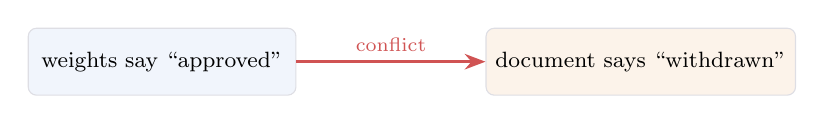
\begin{tikzpicture}[font=\footnotesize, node distance=0.35cm]
      \node[draw=rule, rounded corners=3pt, fill=acquire!8, minimum width=3.4cm, minimum height=0.85cm] (w) {weights say ``approved''};
      \node[draw=rule, rounded corners=3pt, fill=retrieve!10, minimum width=3.4cm, minimum height=0.85cm, right=2.4cm of w] (d) {document says ``withdrawn''};
      \draw[-{Stealth}, update, line width=1pt] (w) -- node[above, font=\scriptsize, text=update] {conflict} (d);
    \end{tikzpicture}
  \end{center}
  \note{Use a real withdrawal, not a toy fact, because the room needs to feel
  that a wrong answer here has a cost. Do not give the result yet. Target:
  75 seconds.}
\end{frame}

% ============================== 6. THE RESULT ================================
\begin{frame}{The measurement}
  \begin{center}
  \begin{tabular}{@{}lrr@{}}
    \toprule
    & \textbf{Without the notice} & \textbf{With the notice in the prompt} \\
    \midrule
    Answers ``safe''      & 37.53\% & \textcolor{update}{\textbf{42.58\%}} \\
    Answers ``withdrawn'' & 0.0004\% & 0.0006\% \\
    Most likely word      & ``safe'' & ``safe'' \\
    \bottomrule
  \end{tabular}
  \end{center}
  \vspace{1.1em}
  \begin{itemize}\setlength\itemsep{0.7em}
    \item The withdrawal notice is \textbf{in the prompt}, and confidence in ``safe'' \textbf{rises}.
    \item The correct answer is left at roughly \textbf{six chances in a million}.
    \item Retrieval succeeded. Resolution failed.
  \end{itemize}
  \note{Pause after 42.58 percent and let the room notice the number went up,
  not down. This is the moment the talk turns. If challenged on cherry-picking:
  the script is deterministic, it is in the repository, and two further cases
  are in the paper. Target: 2 minutes.}
\end{frame}

% ============================== 7. NOT HALLUCINATION =========================
\begin{frame}{This is not hallucination}
  \vspace{0.4cm}
  \begin{center}
    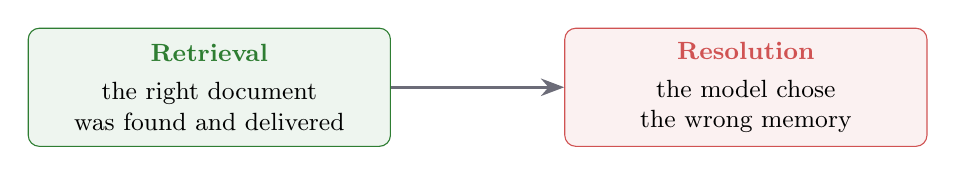
\begin{tikzpicture}[font=\small]
      \node[draw=ok, fill=ok!8, rounded corners=4pt, minimum width=4.6cm, minimum height=1.5cm, align=center] (r)
        {\textcolor{ok}{\textbf{Retrieval}}\\[1mm] the right document\\was found and delivered};
      \node[draw=update, fill=update!8, rounded corners=4pt, minimum width=4.6cm, minimum height=1.5cm, align=center, right=2.2cm of r] (u)
        {\textcolor{update}{\textbf{Resolution}}\\[1mm] the model chose\\the wrong memory};
      \draw[-{Stealth}, line width=1.2pt, muted] (r) -- (u);
    \end{tikzpicture}
  \end{center}
  \vspace{1.0em}
  \begin{center}
    No benchmark for retrieval, editing, or memory tests that second step,\\
    \textbf{because it belongs to none of them}.
  \end{center}
  \note{This slide pre-empts the most common objection, that this is just
  hallucination under another name. It is not: the retriever did its job, and
  the next slide gives the number that proves the context was present and
  ignored. Target: 60 seconds.}
\end{frame}

% ============================== 8. THE METRIC ================================
\begin{frame}{The metric: Lifecycle Desynchronization}
  \begin{equation*}
    \widehat{\mathcal{D}}_{sync}
      = -\ln P\!\left(y^{*} \mid q,\ \theta_{stale},\ \mathcal{M}_{now}\right)
  \end{equation*}
  \vspace{0.4em}
  \begin{itemize}\setlength\itemsep{0.7em}
    \item The surprisal of the \textbf{correct} answer while the corrective document is present.
    \item Measured in nats: $n$ nats means the right answer holds probability $e^{-n}$.
    \item Above $9.2$ nats, no realistic decoding recovers it.
  \end{itemize}
  \vspace{0.8em}
  \begin{center}
    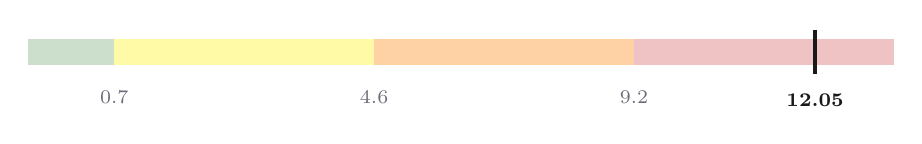
\begin{tikzpicture}
      \fill[ok!25]     (0,0) rectangle (1.1,0.32);
      \fill[yellow!35] (1.1,0) rectangle (4.4,0.32);
      \fill[orange!35] (4.4,0) rectangle (7.7,0.32);
      \fill[update!35] (7.7,0) rectangle (11,0.32);
      \draw[ink, line width=1.6pt] (10.0,-0.12) -- (10.0,0.44);
      \node[font=\scriptsize, text=muted] at (1.1,-0.42) {0.7};
      \node[font=\scriptsize, text=muted] at (4.4,-0.42) {4.6};
      \node[font=\scriptsize, text=muted] at (7.7,-0.42) {9.2};
      \node[font=\scriptsize\bfseries, text=ink] at (10.0,-0.45) {12.05};
    \end{tikzpicture}
  \end{center}
  \note{Explain nats once, in plain terms: it is a log probability, so a bigger
  number means the right answer is buried deeper. The marker on the scale is the
  Vioxx measurement, well past the point where decoding cannot recover.
  Target: 2 minutes.}
\end{frame}

% ============================== 9. THE DIAGNOSTIC ============================
\begin{frame}{Two numbers, not one}
  \vspace{0.2cm}
  \begin{center}
  \small
  \begin{tabular}{@{}lll@{}}
    \toprule
     & \textbf{$\mathcal{I}_{ctx}$ low} & \textbf{$\mathcal{I}_{ctx}$ high} \\
    \midrule
    \textbf{$\mathcal{D}_{sync}$ low}  & \textcolor{ok}{fact never conflicted} & \textcolor{ok}{context resolved the conflict} \\[3pt]
    \textbf{$\mathcal{D}_{sync}$ high} & \textcolor{update}{\textbf{resolution failure}} & \textcolor{retrieve}{drift: influential but losing} \\
    \bottomrule
  \end{tabular}
  \end{center}
  \vspace{1.1em}
  \begin{itemize}\setlength\itemsep{0.6em}
    \item $\mathcal{I}_{ctx}$ measures whether the document moved the model \textbf{at all}.
    \item On Vioxx it is $\mathbf{0.033}$ nats. The document is \textbf{inert}.
    \item That pairing is what separates a broken retriever from a model that ignores what it retrieved.
  \end{itemize}
  \note{This grid is what makes the work a diagnosis rather than a score. High
  D-sync alone is ambiguous: the retriever might have failed. High D-sync with
  near-zero I-ctx is unambiguous. Target: 90 seconds.}
\end{frame}

% ============================== 10. TWO MORE CASES ===========================
\begin{frame}{Three cases, three regimes}
  \vspace{0.2cm}
  \begin{center}
  \small
  \begin{tabular}{@{}lll@{}}
    \toprule
    \textbf{Fact change} & \textbf{What the model does} & \textbf{Regime} \\
    \midrule
    Vioxx withdrawn, 2004      & ignores the notice entirely          & \textcolor{update}{resolution failure} \\[3pt]
    Elizabeth II died, 2022    & the notice boosts ``Queen''          & \textcolor{retrieve}{the exposure trap} \\[3pt]
    Twitter renamed X, 2023    & moves hard, still answers ``Twitter'' & \textcolor{store}{drift} \\
    \bottomrule
  \end{tabular}
  \end{center}
  \vspace{1.1em}
  \begin{center}
    The middle row is the uncomfortable one: \textbf{a correct document made the wrong answer stronger.}
  \end{center}
  \note{The monarch case is the one researchers remember, so give it a beat.
  Telling the model that Elizabeth II died raises the probability of the word
  Queen, because mentioning a fact, even to correct it, reinforces the
  association. Target: 90 seconds.}
\end{frame}

% ============================== 11. THE CAUSE ================================
\begin{frame}{The cause: storage discards provenance}
  \begin{itemize}\setlength\itemsep{0.9em}
    \item Training teaches a model \textbf{what} is true.
    \item It never records \textbf{when} the fact was learned, or \textbf{where} it came from.
    \item So at inference there is no principled basis for preferring fresh evidence
          over a confident old memory.
  \end{itemize}
  \vspace{1.0em}
  \begin{center}
    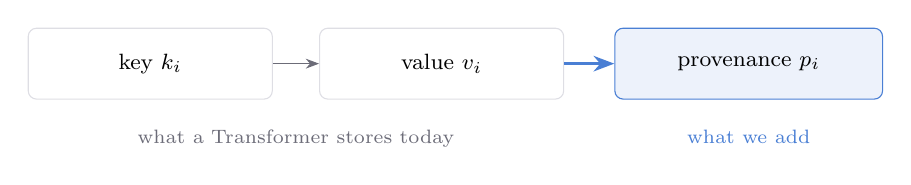
\begin{tikzpicture}[font=\footnotesize]
      \node[draw=rule, rounded corners=3pt, minimum width=3.1cm, minimum height=0.9cm] (k) at (0,0) {key $k_i$};
      \node[draw=rule, rounded corners=3pt, minimum width=3.1cm, minimum height=0.9cm] (v) at (3.7,0) {value $v_i$};
      \node[draw=acquire, fill=acquire!10, rounded corners=3pt, minimum width=3.4cm, minimum height=0.9cm] (p) at (7.6,0) {provenance $p_i$};
      \draw[-{Stealth}, muted] (k) -- (v);
      \draw[-{Stealth}, acquire, line width=1pt] (v) -- (p);
      \node[below, text=muted, font=\scriptsize] at (1.85,-0.72) {what a Transformer stores today};
      \node[below, text=acquire, font=\scriptsize] at (7.6,-0.72) {what we add};
    \end{tikzpicture}
  \end{center}
  \note{This is the pivot from diagnosis to proposal. The room should agree that
  the missing ingredient is metadata before seeing any mechanism. Target:
  90 seconds.}
\end{frame}

% ============================== 12. THE PROPOSAL =============================
\begin{frame}{The proposal: gate stale facts at inference}
  \begin{equation*}
    \text{FFN}_{steered}(x) \;=\; \sum_{i=1}^{d_m} S(\Delta\tau_i)\ f(x \cdot k_i)\ v_i,
    \qquad
    S(\Delta\tau_i) = \sigma\!\left(\gamma - \beta \cdot \Delta\tau_i\right)
  \end{equation*}
  \vspace{0.5em}
  \begin{itemize}\setlength\itemsep{0.7em}
    \item Fresh facts pass with $S \approx 1$; stale facts are attenuated toward $0$.
    \item \textbf{The weights are never modified}, so the specificity bottleneck that
          limits static editing does not apply.
    \item Cost: about $1$M parameters on a 7B model, under $\mathbf{0.02\%}$.
  \end{itemize}
  \vspace{0.7em}
  \begin{center}\color{muted}\small
    Think of it as a volume control on every stored fact, turned down by age.
  \end{center}
  \note{The volume-knob analogy works better than the equation for a mixed
  audience, so say the analogy first and let the equation confirm it. Target:
  2 minutes.}
\end{frame}

% ============================== 13. HONESTY ==================================
\begin{frame}{What is measured, and what is proposed}
  \vspace{0.4cm}
  \begin{center}
    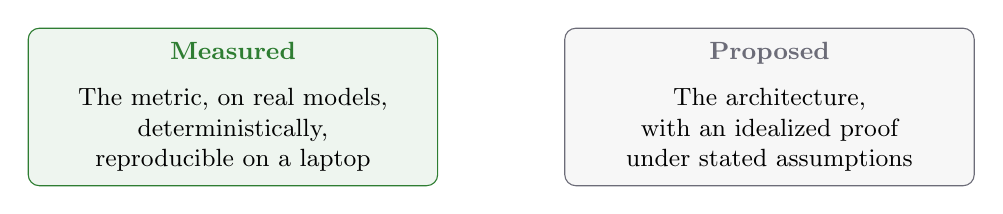
\begin{tikzpicture}[font=\small]
      \node[draw=ok, fill=ok!8, rounded corners=4pt, minimum width=5.2cm, minimum height=2.0cm, align=center] (m)
        {\textcolor{ok}{\textbf{Measured}}\\[2mm] The metric, on real models,\\deterministically,\\reproducible on a laptop};
      \node[draw=muted, fill=black!3, rounded corners=4pt, minimum width=5.2cm, minimum height=2.0cm, align=center, right=1.6cm of m] (p)
        {\textcolor{muted}{\textbf{Proposed}}\\[2mm] The architecture,\\with an idealized proof\\under stated assumptions};
    \end{tikzpicture}
  \end{center}
  \vspace{0.9em}
  \begin{center}
    The Provenance Vector has \textbf{not} been trained. It needs a pretraining run,\\
    and the paper says so in its limitations rather than leaving you to find out.
  \end{center}
  \note{Say this before anyone asks. Volunteering the limitation buys credibility
  for everything else in the talk, and it removes the sharpest question a jury
  can put to you. Target: 60 seconds.}
\end{frame}

% ============================== 14. REPRODUCIBILITY ==========================
\begin{frame}{Check it yourself}
  \vspace{0.4cm}
  \begin{itemize}\setlength\itemsep{0.9em}
    \item Every number in this talk comes from \textbf{one deterministic script}.
          No sampling, identical digits on any machine.
    \item The model is GPT-2 base, 124M parameters: small, fully open, and free of
          instruction tuning that would confound the result.
    \item The demonstration runs GPT-2 \textbf{inside your browser}. Nothing you type
          leaves your laptop.
  \end{itemize}
  \vspace{1.2em}
  \begin{center}\footnotesize
    \textbf{Paper and code}\quad \href{https://github.com/Amey-Thakur/LLM-KNOWLEDGE-LIFECYCLE}{github.com/Amey-Thakur/LLM-KNOWLEDGE-LIFECYCLE}\\[2.5mm]
    \textbf{Live demonstration}\quad \href{https://huggingface.co/spaces/ameythakur/llm-knowledge-lifecycle}{huggingface.co/spaces/ameythakur/llm-knowledge-lifecycle}
  \end{center}
  \note{If there is a screen and a minute to spare, open the demo live and run
  the Vioxx probe. A measurement performed in front of the room is worth more
  than any slide. Target: 90 seconds, or 2 minutes with the live run.}
\end{frame}

% ============================== 15. WHAT NEXT ================================
\begin{frame}{What comes next}
  \begin{itemize}\setlength\itemsep{0.9em}
    \item \textbf{Does it survive scale?} A cross-model sweep across six open models
          is prepared and running.
    \item \textbf{Does instruction tuning fix it?} Chat-tuned models follow context
          more readily; whether that closes the gap is an open question.
    \item \textbf{Does reasoning-mode inference help?} Extended test-time compute
          should, in principle, resolve conflicts the forward pass cannot.
    \item \textbf{Multimodal.} A text prior overriding a contradicting image is the
          same failure in another modality.
  \end{itemize}
  \vspace{0.8em}
  \begin{center}\color{muted}\small
    An honest null result answers the first question just as usefully as a positive one.
  \end{center}
  \note{Be plain that the sweep is running and we will report whatever it says.
  Committing publicly to reporting a null result is itself a credibility signal
  to a jury. Target: 90 seconds.}
\end{frame}

% ============================== 16. SUMMARY ==================================
\begin{frame}{In three sentences}
  \vspace{1.0cm}
  \begin{itemize}\setlength\itemsep{1.3em}
    \item Five separate research fields are five stages of \textbf{one lifecycle},
          and systems fail at the boundaries nobody benchmarks.
    \item Those failures are \textbf{measurable}: a model with the correction in its
          prompt still answers wrong, at 12.05 nats.
    \item The cause is that storage \textbf{discards provenance}, and an inference-time
          gate can address it without touching the weights.
  \end{itemize}
  \vspace{1.2em}
  \begin{center}
    
\begin{tikzpicture}
      \foreach \c/\n [count=\i from 0] in
        {acquire/Acquire, store/Store, retrieve/Retrieve, update/Update, forget/Forget}
        \node[fill=\c, text=white, font=\scriptsize\bfseries, rounded corners=2pt,
              minimum width=1.9cm, minimum height=0.55cm] at (\i*2.05, 0) {\n};
    \end{tikzpicture}
  \end{center}
  \note{If you are running short, this slide can carry the last three minutes on
  its own. Say each bullet once, without elaborating, then go to questions.
  Target: 60 seconds.}
\end{frame}

% ============================== 17. THANK YOU ================================
\begin{frame}[plain]
  \vspace{1.3cm}
  \begin{center}
    {\Large\bfseries Thank you}\\[3mm]
    {\color{muted}\small Questions}\\[10mm]

    \begin{tikzpicture}
      \begin{scope}\clip (0,0) circle (0.8cm);
        \node at (0,0) {
\includegraphics[width=1.6cm]{amey-thakur.jpg}};\end{scope}
      \draw[rule, line width=1pt] (0,0) circle (0.8cm);
      \node[below, font=\footnotesize\bfseries] at (0,-0.95) {Amey Thakur};
      \node[below, font=\tiny, text=muted] at (0,-1.3) {\href{mailto:ameythakur20@gmail.com}{ameythakur20@gmail.com}};

      \begin{scope}\clip (5.2,0) circle (0.8cm);
        \node at (5.2,0) {
\includegraphics[width=1.6cm]{sarvesh-talele.jpg}};\end{scope}
      \draw[rule, line width=1pt] (5.2,0) circle (0.8cm);
      \node[below, font=\footnotesize\bfseries] at (5.2,-0.95) {Sarvesh Talele};
      \node[below, font=\tiny, text=muted] at (5.2,-1.3) {\href{mailto:talelesarvesh@gmail.com}{talelesarvesh@gmail.com}};
    \end{tikzpicture}\\[7mm]

    {\scriptsize\href{https://github.com/Amey-Thakur/LLM-KNOWLEDGE-LIFECYCLE}{github.com/Amey-Thakur/LLM-KNOWLEDGE-LIFECYCLE}}
  \end{center}
  \note{Leave this slide up for the whole question period so the contact details
  and repository stay visible. The backup slide follows if a question needs it.}
\end{frame}

% ============================== 18. BACKUP ===================================
\begin{frame}{Backup: anticipated questions}
  \vspace{0.2cm}
  \small
  \begin{itemize}\setlength\itemsep{0.75em}
    \item \textbf{Why GPT-2 and not a frontier model?} Small, fully open, no
          instruction-tuning confound, and it makes the result checkable on a laptop.
          The claim is that the failure exists and is measurable, not that it is universal.
    \item \textbf{Is this just hallucination?} No. The retriever succeeded, and
          $\mathcal{I}_{ctx} = 0.033$ proves the context was present and inert.
    \item \textbf{Does it disappear at scale?} Unknown, and that is the honest answer.
          The sweep is running; we will report what it shows.
    \item \textbf{Why not just edit the weights?} Editing damages neighboring facts,
          and degrades as edits accumulate. Gating leaves the weights untouched.
    \item \textbf{Is the proof meaningful if untrained?} It shows the mechanism is
          structurally sound given accurate provenance. The assumptions are stated,
          not hidden.
  \end{itemize}
  \note{Do not show this slide unless a question calls for it. Knowing it is
  there is what keeps you calm during questions.}
\end{frame}

\end{document}
